% !TeX spellcheck = en_US

\section{Preprocessing} \label{sec:preprocessing}

\subsection{Data cleaning} \label{sec:data-clean}

As the first thing we did with our datasets, we just applied the data cleaning by Hou, Saha and Tsang [\ref{Hou}] with some adaptation to our purpose, e.g., we want to consider restaurants in all the available cities and not only Las Vegas.

What we do based on their kernel is:
\begin{enumerate}
	\item Transfer json into Pandas dataframe with proper indexing;
	\item Extract data that includes all restaurants;
	\item Replace garbage data which includes incorrect states and postal codes;
	\item Date transformations and standardization;
	\item Create new explanatory features based on initial features;
	\item Delete consequently unnecessary columns which could add ambiguity based on new features;
	\item Delete duplicate restaurants entries and combine their reviews;
	\item Save obtained datasets in pickle format so that they occupy less space in memory.
\end{enumerate}

The main features they work on are \texttt{categories}, \texttt{attributes} and \texttt{hours} in the \textit{business} dataset, renamed \textit{restaurants} since other kind of businesses are not considered.\\
The feature \texttt{categories} contains a list of kinds of businesses, ranging from shops to sport centers, so only the items that contains \texttt{"restaurant"} in that list are kept; then the most frequent and significant categories are extracted and saved in a new feature called \texttt{cuisine}, that we used to infer the users' preferences and to compute the historical features [\ref{sec:hist-feat}].\\
The feature \texttt{attributes} contains a dictionary of characteristics of the restaurant, such as if it offers alcohol or if it has wifi connection, but these dictionaries are a bit messy, so the authors create a new feature for each attribute and make the values homogeneous, for example \texttt{wifi} has values such as \texttt{"No", "u`no'", "`no'", `None'} and only \texttt{"No"} is kept.\\
The feature \texttt{hours} contains a dictionary of the form \texttt{\{"day\_of\_the\_week": "opening\_hour-closing\_hour"\}}, so it's not very usable, thus the authors divide this features in two features per day of the week: one for the opening and one for the closing.


\subsection{Fake Review Detection} \label{sec:fake-rev}

With our data clean and tidy, we used some models described by Zhang in [\ref{Zhang}] to detect deceptive reviews and associate a \textit{trustworthiness score} to each of them.

We trained all of their models: a Convolutional Neural Network, fed with sequences obtained by a tokenizer from the \href{https://keras.io/preprocessing/text/}{Keras preprocessing} library, and a Support Vector Machine, fitted on vectors computer by Scikit Learn's \href{https://scikit-learn.org/stable/modules/generated/sklearn.feature_extraction.text.TfidfVectorizer.html}{TfidfVectorizer}.\\
It turned out that the performances of the Convolutional Neural Network were worse \wrt the Support Vector Machine, as we can see in the tables [\ref{tab:cnn-fake-rev}] and [\ref{tab:svm-fake-rev}].

\begin{table}[h]
	\centering
	\begin{tabular}{lllll}
		\rowcolor[HTML]{EEEEEE} 
		\cellcolor[HTML]{FBFBFB} & \textbf{precision} & \textbf{recall} & \textbf{f1-score} & \textbf{support} \\
		\rowcolor[HTML]{EEEEEE} 
		\textbf{-1}              & 0.18               & 0.18            & 0.18              & 24070            \\
		\rowcolor[HTML]{EEEEEE} 
		\textbf{+1}              & 0.87               & 0.88            & 0.88              & 158468           \\
		\rowcolor[HTML]{FBFBFB} 
		&                    &                 &                   &                  \\
		\rowcolor[HTML]{EEEEEE} 
		\textbf{micro avg}       & 0.78               & 0.78            & 0.78              & 182538           \\
		\rowcolor[HTML]{EEEEEE} 
		\textbf{macro avg}       & 0.53               & 0.53            & 0.53              & 182538           \\
		\rowcolor[HTML]{EEEEEE} 
		\textbf{weighted avg}    & 0.78               & 0.78            & 0.78              & 182538           \\
		\rowcolor[HTML]{FBFBFB} 
		&                    &                 &                   &                  \\
		\rowcolor[HTML]{EEEEEE} 
		\textbf{accuracy}        & \multicolumn{4}{l}{\cellcolor[HTML]{EEEEEE}78.3\%}                         
	\end{tabular}
	\caption{Report for CNN model for fake review detection}
	\label{tab:cnn-fake-rev}
\end{table}

\begin{table}[h]
	\centering
	\begin{tabular}{lllll}
		\rowcolor[HTML]{EEEEEE} 
		\cellcolor[HTML]{FBFBFB} & \textbf{precision} & \textbf{recall} & \textbf{f1-score} & \textbf{support} \\
		\rowcolor[HTML]{EEEEEE} 
		\textbf{-1}              & 0.84               & 0.95            & 0.89              & 161016           \\
		\rowcolor[HTML]{EEEEEE} 
		\textbf{+1}              & 0.96               & 0.86            & 0.91              & 211105           \\
		\rowcolor[HTML]{FBFBFB} 
		&                    &                 &                   &                  \\
		\rowcolor[HTML]{EEEEEE} 
		\textbf{micro avg}       & 0.90               & 0.90            & 0.90              & 372121           \\
		\rowcolor[HTML]{EEEEEE} 
		\textbf{macro avg}       & 0.90               & 0.91            & 0.90              & 372121           \\
		\rowcolor[HTML]{EEEEEE} 
		\textbf{weighted avg}    & 0.91               & 0.90            & 0.90              & 372121           \\
		\rowcolor[HTML]{FBFBFB} 
		&                    &                 &                   &                  \\
		\rowcolor[HTML]{EEEEEE} 
		\textbf{accuracy}        & \multicolumn{4}{l}{\cellcolor[HTML]{EEEEEE}89.99\%}                        
	\end{tabular}
	
	\caption{Report for SVM model for fake review detection}
	\label{tab:svm-fake-rev}
\end{table}

Thus, we used the SVM to compute predictions and establish which reviews are reliable and which are deceptive, in a binary fashion, so we added to the review dataset a feature \texttt{bin\_truth\_score} that holds a 1 for true reviews and a -1 for fake ones.

In order to have a probability distribution instead of a binary result, the SVM is passed as a parameter to a Scikit Learn's \href{https://scikit-learn.org/stable/modules/generated/sklearn.calibration.CalibratedClassifierCV.html}{CalibratedClassifierCV}, whose predictions are the probabilities that a review is authentic, instead of binary results, and we used them to add a feature \texttt{real\_truth\_score} to the review dataset.

Once this was done, we removed the texts of the reviews.

In the figures [\ref{fig:SVC-truth-labels}] and [\ref{fig:calibrated-truth-labels}] we can see the distribution of the two kinds of labels.

\begin{figure}[h!]
	\centering
	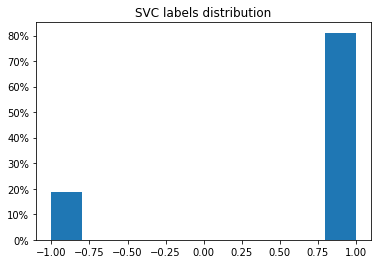
\includegraphics[scale=0.6]{SVC_truth_labels}
	\caption{SVC truth labels}
	\label{fig:SVC-truth-labels}
\end{figure}

\begin{figure}[h!]
	\centering
	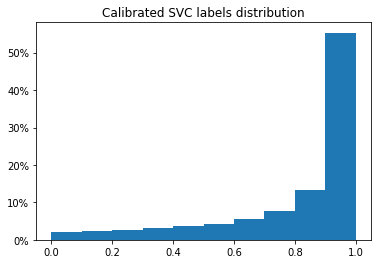
\includegraphics[scale=0.6]{calibrated_truth_labels}
	\caption{Calibrated truth labels}
	\label{fig:calibrated-truth-labels}
\end{figure}


\subsection{Historical features}\label{sec:hist-feat}

Based on Gandhe's paper [\ref{Gandhe}], we have added some \textit{historical features} to our dataset:
\begin{enumerate}
	\item User-level features:
	\begin{enumerate}
		\item average of the ratings given by a certain user,
		\item number of reviews written by a certain user;
	\end{enumerate}
	\item Business-level features: 
	\begin{enumerate}
		\item average of the ratings given to a certain restaurant,
		\item number of reviews written about a certain restaurant;
	\end{enumerate}
	\item User-business-level features: 
	\begin{enumerate}
		\item average rating given by a certain user to each cuisine (feature defined in section \nameref{sec:data-clean}), i.e., for each cuisine, the average of all the votes given by a user to all the restaurants that contains that cuisine in their list,
		\item average of the ratings given by a certain user to the cuisines of a certain restaurant, i.e., the average of the votes given by a user to the cuisines present in the list of a restaurant, as computed in the feature (3.1.).
	\end{enumerate}
\end{enumerate}

In order to do this, we had to split the review dataset in three parts:
\begin{itemize}
	\item \textit{Test set}, from the last day considered in the dataset, to the previous $m$ months;
	\item \textit{Training set}, from the day before the beginning of the test set, up to $n$ months before;
	\item \textit{History}, the remaining part of the dataset, used to compute historical features.
\end{itemize}
We have picked $m=3$ and $n=8$, so the test set goes from 9/1/2018 to 11/30/2018, the training set goes from 1/1/2018 to 8/31/2018, the history contains the remaining data, from 10/12/2004 to 12/31/2017.

While the other features were quite straightforward to implement and fast to compute, we had to optimize the code of the feature (3.1.) in order to prevent its computation from taking more days, so we tried two libraries that are supposed to automatically speed up a python program running it on more processors, with a minimal intervention by the programmer. The first, \href{https://modin.readthedocs.io/en/latest/index.html}{Modin}, is specifically meant for Pandas, and the second, \href{https://numba.pydata.org/}{Numba}, more generically for Python math operations, but none of them actually worked, the former because of some incompatibility with Windows OS, and the latter because it ``likes NumPy'' (as written \href{http://numba.pydata.org/numba-doc/latest/user/5minguide.html#will-numba-work-for-my-code}{in the docs}) but not Pandas. So, we decided to manually split the datasets and pass portions of them to a function launched in parallel on multiple processors by a \href{https://docs.python.org/3.6/library/multiprocessing.html#module-multiprocessing.pool}{process pool}, and this reduced the computation time to just few hours.

We decided to apply our two estimators of the trustworthiness of the reviews (described in \nameref{sec:fake-rev}) to compute two additional version of the just described features, so we have three flavors for each of these features:
\begin{enumerate}
	\item \textit{standard}: each review is treated in the same way (every review has weight 1),
	\item \textit{binary}: the authentic reviews have weight 1 and the deceptive ones have weight 0, accordingly to their \texttt{bin\_truth\_score}, so fake reviews aren't counted in total or average,
	\item \textit{real}: each review is weighted with its \texttt{real\_truth\_score}, both for the total and for the average.
\end{enumerate}


\subsection{User-based collaborative approach}\label{sec:coll-appr}

Then, we decided to add a new feature based on \textit{collaborative filtering}: the idea is that we have lots of reviews written by lots of users, so we can use the score given by similar user to similar restaurants to predict what a certain user will think about a restaurant he never tried before.
So we applied the following formula:
\begin{equation}
    pred(u, r) = a_u + \frac{\sum_{u_i \in U} sim(u, u_i) * \left( a_{u_i, r} - a_r \right)} {\sum_{u_i \in U} sim(u, u_i)}
\end{equation}
where
\begin{itemize}
	\item[-] $a_u$ is the average of the votes given by the user $u$ to all the restaurants that share some cuisines with $r$ (i.e., the feature 3.2. between user $u$ and restaurant $r$ defined in section \nameref{sec:hist-feat}),
	\item[-] $U$ is the set of all the users in the dataset, $u$ excluded,
	\item[-] $a_{u_i, r}$ is the same as $a_u$, but for user $u_i$, so it is the value of the feature 3.2. for user $u_i$ and restaurant $r$,
	\item[-] $a_r$ is the average rating received by $r$ (i.e., the feature 2.1.),
	\item[-] $sim(u, u_i)$ is computed as the cosine similarity between two vectors that represent the two users $u$ and $u_i$, composed by the values for the features 3.1. (one for each cuisine and one for each version, as explained in \nameref{sec:hist-feat}).
\end{itemize}

We have three versions for this feature too, with the same meaning described in the previous section.

\subsection{Dimensionality reduction and further preprocessing}

At this point we had all the features we needed, so, that was the moment of preparing the data so that they were ready to be fed to the models. The next steps we performed were the following:
\begin{enumerate}
	\item We joined all the interesting datasets in only one, to have all the needed features together and one review per row (the \textit{checkin} dataset was discarded because not useful);
	\item We added the label \texttt{likes} that holds a 1 if that user gave 4 or 5 stars in that review or 0 if he/she gave 1, 2 or 3 stars;
	\item We removed unnecessary columns sush as \texttt{review date, restaurant name, restaurant address, user name};
	\item We applied some dimensionality reduction (more details on this later);
	\item We filled missing values with the mode of the feature for the categorical values and with the mean for the numerical ones;
	\item We converted categorical features into numerical features, readable by the models:
	\begin{itemize}
		\item for the features \texttt{OutdoorSeating, BusinessAcceptsCreditCards, RestaurantsDelivery, RestaurantsReservations, WiFi, Alcohol, city} we used Pandas' \href{https://pandas.pydata.org/pandas-docs/stable/reference/api/pandas.get_dummies.html}{\texttt{get\_dummies()}} function, that applies one hot encoding on the input features,
		\item for the features \texttt{Monday\_Open, Tuesday\_Open, Wednesday\_Open, Thursday\_Open,\\ Friday\_Open, Saturday\_Open, Sunday\_Open, Monday\_Close, Tuesday\_Close,\\ Wednesday\_Close, Thursday\_Close,Friday\_Close, Saturday\_Close, Sunday\_Close,\\ postal\_code} we applied Scikit learn's \href{https://scikit-learn.org/stable/modules/generated/sklearn.preprocessing.OrdinalEncoder.html}{\texttt{OrdinalEncoder.fit\_transform()}}, that encodes categorical features as an integer array: it could bias the models but it is less memory consuming \wrt one hot encoding, so we preferred this method for features that we consider less determinant and that have many possible values.
	\end{itemize}
\end{enumerate}

Since our dataset was huge (about 7GB), we decided to apply some dimensionality reduction in order to make it fit in RAM, especially when applying grid search (it turned out that to make parallelism more efficient the Scikit Learn's method for grid search tries to make a copy of the dataset for each parallel job that it runs).\\
We had two features that seem to be quite important and that could assume hundreds of values: \texttt{city} and \texttt{categories}.
First of all, we plotted the distribution of the values of these features, as shown in the figures [\ref{fig:city-distribution}] and [\ref{fig:category-distribution}]: it appears that there are few very frequent values (such as \texttt{'Las Vegas', 'Phoenix', 'Toronto'} for the cities and \texttt{'Food', 'Nightlife', 'Bars'} for the categories) and lots of values that are pretty rare, thus we decided to cut the less frequent values before proceeding with one hot encoding, so we choose a threshold $\theta=100$ and replaced all the values that occur less than $\theta$ times with \texttt{'other'}.\\
Let's note that, since after one hot encoding we have one column for each category, the previously created \texttt{cuisine} feature (see \nameref{sec:data-clean} section) has become useless, so we removed it.\\
In the tables [\ref{tab:city-frequencies}] and [\ref{tab:category-frequencies}] are listed the ten most frequent and ten least frequent cities/categories.

\begin{figure}[h!]
	\centering
	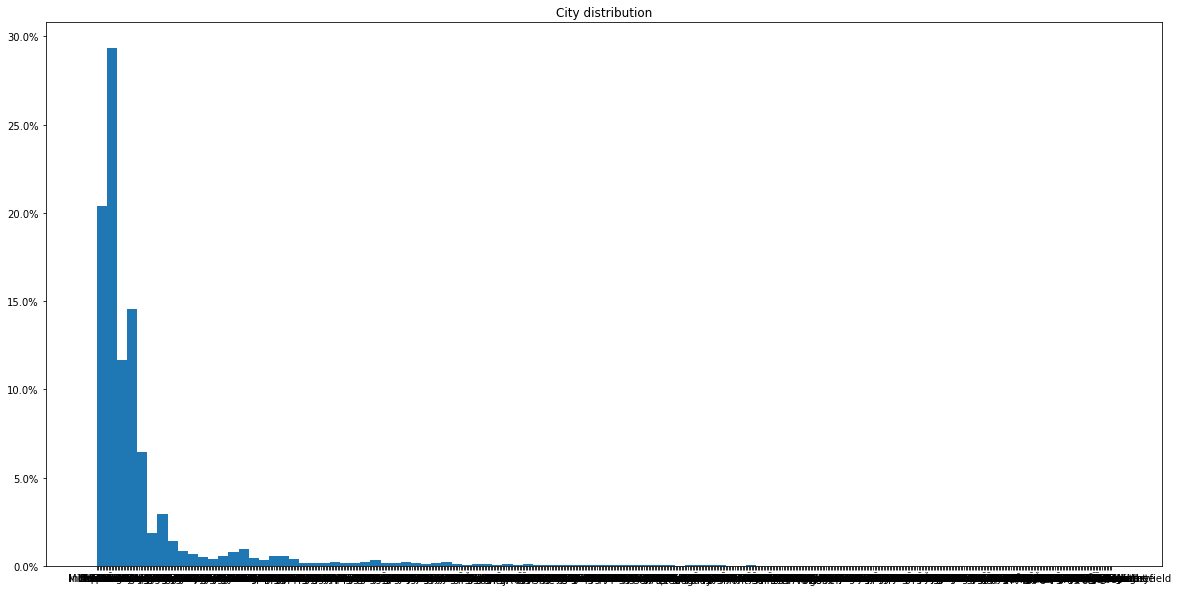
\includegraphics[scale=0.4]{city_distribution}
	\caption{City distribution}
	\label{fig:city-distribution}
\end{figure}

\begin{figure}[h!]
	\centering
	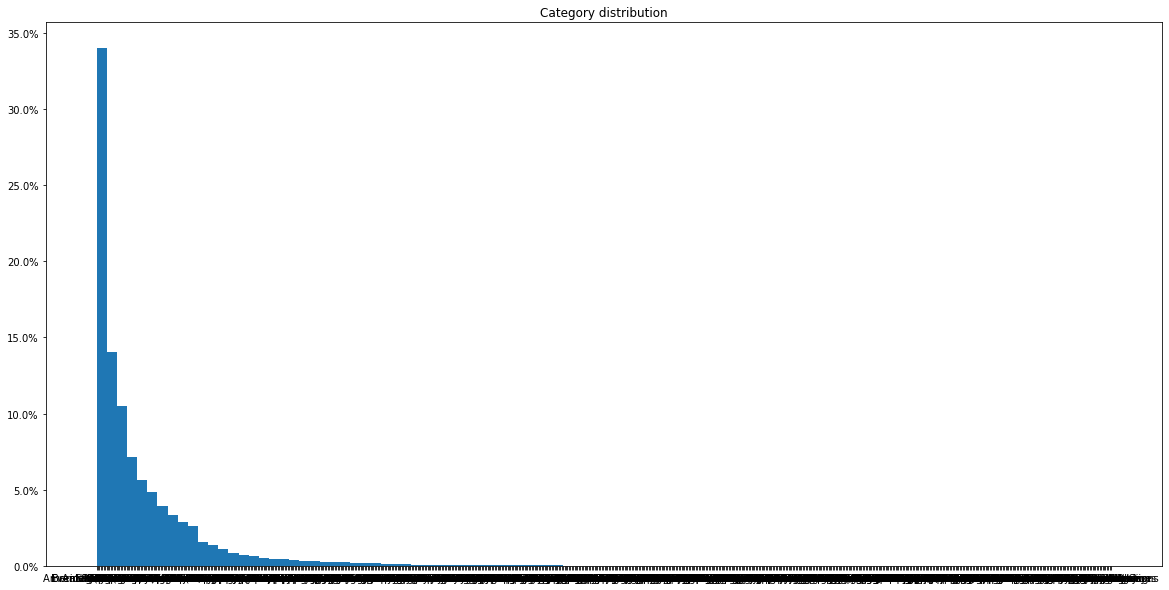
\includegraphics[scale=0.4]{category_distribution}
	\caption{Category distribution}
	\label{fig:category-distribution}
\end{figure}

\newpage

\begin{table}[h!]
	\parbox{.45\linewidth}{
		\centering
		\begin{tabular}{
				>{\columncolor[HTML]{EEEEEE}}l 
				>{\columncolor[HTML]{EEEEEE}}l }
			\textbf{city} & \textbf{\# occurrences} \\ \hline
			Las Vegas	        	& 208437 \\ 
			Phoenix	            	& 71126 \\ 
			Toronto	            	& 57047 \\ 
			Charlotte		        & 40190 \\ 
			Scottsdale	        	& 36579 \\ 
			Pittsburgh	        	& 26891 \\ 
			Henderson	        	& 21518 \\ 
			Montreal	        	& 18531 \\ 
			Tempe	               	& 18354 \\ 
			Mesa	            	& 17235 \\ 
			...                     & ... \\ 
			Paw Creek		        & 1 \\ 
			Tottenham	        	& 1 \\ 
			springdale	        	& 1 \\ 
			Coteau-du-Lac	    	& 1 \\ 
			Huntingdon	        	& 1 \\ 
			Fabreville	        	& 1 \\ 
			De Winton	        	& 1 \\ 
			Napierville		        & 1 \\ 
			Laval, Ste Dorothee		& 1 \\
			Les Coteaux             & 1
		\end{tabular}
		\caption{City frequencies}
		\label{tab:city-frequencies}
	}
	\hfill
	\parbox{.45\linewidth}{
		\centering
		\begin{tabular}{
				>{\columncolor[HTML]{EEEEEE}}l 
				>{\columncolor[HTML]{EEEEEE}}l }
			\textbf{category} & \textbf{\# occurrences} \\ \hline
			Food                            & 192841 \\ 
			Nightlife                       & 170259 \\ 
			Bars                            & 165959 \\ 
			American (Traditional)          & 123975 \\ 
			Breakfast \& Brunch             & 120310 \\ 
			American (New)                  & 117437 \\ 
			Sandwiches                      & 82264 \\ 
			Mexican                         & 73726 \\ 
			Burgers                         & 71598 \\ 
			Pizza                           & 67538 \\ 
			...                             & ...   \\ 
			Beer Hall                       & 1 \\ 
			Banks \& Credit Unions          & 1 \\ 
			University Housing              & 1 \\ 
			Pet Groomers                    & 1 \\ 
			Gardeners                       & 1 \\ 
			Home Health Care                & 1 \\ 
			Campgrounds                     & 1 \\ 
			Holiday Decorations             & 1 \\ 
			Roofing                         & 1 \\ 
			Senegalese                      & 1
		\end{tabular}
		\caption{Category frequencies}
		\label{tab:category-frequencies}
	}
\end{table}

When parameter tuning was finished and grid search wasn't needed anymore, we tried to fit the obtained models with the original dataset, without applying dimensionality reduction and restricting the potentially dangerous use of \texttt{OrdinalEncoder} \texttt{postal\_code} only, in order to see if we could get some improvement in performances of the models.\\
The procedure we followed and the results we obtained are explained in more detail in section \nameref{sec:experiments}.
